\documentclass[11pt,a4paper]{article}

% ============================================================================
% PACKAGES
% ============================================================================
\usepackage[utf8]{inputenc}
\usepackage[T1]{fontenc}
\usepackage{amsmath,amssymb,amsthm}
\usepackage{mathtools}
\usepackage{bm}
\usepackage{algorithm}
\usepackage{algorithmic}
\usepackage{booktabs}
\usepackage{multirow}
\usepackage{array}
\usepackage{graphicx}
\usepackage{xcolor}
\usepackage{hyperref}
\usepackage{tikz}
\usetikzlibrary{shapes,arrows,positioning,calc,patterns,decorations.pathreplacing}
\usepackage{pgfplots}
\pgfplotsset{compat=1.17}
\usepackage{listings}
\usepackage{tcolorbox}
\usepackage{enumitem}
\usepackage{geometry}
\geometry{margin=1in}

% ============================================================================
% THEOREM ENVIRONMENTS
% ============================================================================
\theoremstyle{definition}
\newtheorem{definition}{Definition}[section]
\newtheorem{example}{Example}[section]
\newtheorem{remark}{Remark}[section]

\theoremstyle{plain}
\newtheorem{theorem}{Theorem}[section]
\newtheorem{proposition}{Proposition}[section]
\newtheorem{lemma}{Lemma}[section]
\newtheorem{corollary}{Corollary}[section]

% ============================================================================
% CUSTOM COMMANDS
% ============================================================================
\newcommand{\R}{\mathbb{R}}
\newcommand{\E}{\mathbb{E}}
\newcommand{\Var}{\text{Var}}
\newcommand{\Cov}{\text{Cov}}
\newcommand{\N}{\mathcal{N}}
\newcommand{\SI}{\text{SI}}
\newcommand{\MSI}{\text{MSI}}
\newcommand{\argmax}{\operatornamewithlimits{argmax}}
\newcommand{\argmin}{\operatornamewithlimits{argmin}}

% Code listing style
\lstset{
    language=Python,
    basicstyle=\ttfamily\small,
    keywordstyle=\color{blue},
    commentstyle=\color{gray},
    stringstyle=\color{red},
    numbers=left,
    numberstyle=\tiny\color{gray},
    frame=single,
    breaklines=true,
    captionpos=b
}

% Colored boxes for intuition
\newtcolorbox{intuition}[1][]{
    colback=blue!5!white,
    colframe=blue!75!black,
    fonttitle=\bfseries,
    title=Intuition,
    #1
}

\newtcolorbox{keypoint}[1][]{
    colback=green!5!white,
    colframe=green!50!black,
    fonttitle=\bfseries,
    title=Key Point,
    #1
}

\newtcolorbox{warning}[1][]{
    colback=red!5!white,
    colframe=red!75!black,
    fonttitle=\bfseries,
    title=Important,
    #1
}

% ============================================================================
% DOCUMENT
% ============================================================================
\title{\Huge\textbf{Emergent Specialization in Multi-Agent Systems}\\[0.5cm]
\Large A Comprehensive Mathematical Deep Dive into the Method}

\author{Companion Document to the NeurIPS Paper\\[0.3cm]
\textit{For readers with strong mathematical background}}

\date{\today}

\begin{document}

\maketitle

\begin{abstract}
This document provides an exhaustive, ground-up explanation of the NichePopulation algorithm and the theory of emergent specialization in multi-agent systems. We combine rigorous mathematical treatment with intuitive explanations, worked examples, code implementations, and visualizations. The document is designed for readers with a strong mathematical background who want to understand every detail of how and why agents spontaneously specialize under competitive pressure.

\textbf{Prerequisites:} Basic probability theory, linear algebra, and familiarity with optimization. All other concepts (information theory, game theory, Bayesian inference) are developed from first principles.
\end{abstract}

\tableofcontents
\newpage

% ============================================================================
% PART I: FOUNDATIONS
% ============================================================================
\part{Mathematical Foundations}

Before diving into the algorithm, we establish the mathematical toolkit required to understand emergent specialization. This includes information theory (for measuring specialization), game theory (for understanding competitive dynamics), and Bayesian inference (for learning under uncertainty).

\section{Information Theory Foundations}

\subsection{Shannon Entropy: Measuring Uncertainty}

Information theory, developed by Claude Shannon in 1948, provides the mathematical framework for quantifying uncertainty and information content in probability distributions.

\begin{definition}[Shannon Entropy]
For a discrete random variable $X$ with probability mass function $p(x)$ over a finite alphabet $\mathcal{X}$, the \textbf{Shannon entropy} is defined as:
\begin{equation}
H(X) = -\sum_{x \in \mathcal{X}} p(x) \log p(x)
\end{equation}
where we adopt the convention that $0 \log 0 = 0$ (justified by the limit $\lim_{p \to 0^+} p \log p = 0$).
\end{definition}

\begin{intuition}
Entropy measures the ``average surprise'' when sampling from a distribution:
\begin{itemize}
    \item If outcomes are predictable (one outcome dominates), entropy is \textbf{low}
    \item If outcomes are unpredictable (uniform distribution), entropy is \textbf{high}
\end{itemize}
\end{intuition}

\subsubsection{Units and Logarithm Base}

The choice of logarithm base determines the unit of entropy:
\begin{itemize}
    \item $\log_2$: entropy measured in \textbf{bits}
    \item $\ln$ (natural log): entropy measured in \textbf{nats}
    \item $\log_{10}$: entropy measured in \textbf{dits} (decimal digits)
\end{itemize}

Throughout this document, we use natural logarithm ($\ln$), so entropy is measured in nats. The conversion is: $H_{\text{bits}} = H_{\text{nats}} / \ln(2) \approx 1.443 \cdot H_{\text{nats}}$.

\subsubsection{Properties of Entropy}

\begin{proposition}[Properties of Shannon Entropy]
Let $X$ be a discrete random variable over $\mathcal{X}$ with $|\mathcal{X}| = n$. Then:
\begin{enumerate}
    \item \textbf{Non-negativity}: $H(X) \geq 0$
    \item \textbf{Zero entropy}: $H(X) = 0$ if and only if $X$ is deterministic (one outcome has probability 1)
    \item \textbf{Maximum entropy}: $H(X) \leq \log n$, with equality if and only if $X$ is uniformly distributed
\end{enumerate}
\end{proposition}

\begin{proof}
\textbf{(1) Non-negativity:} Since $p(x) \in [0,1]$, we have $\log p(x) \leq 0$. Thus $-p(x) \log p(x) \geq 0$ for all $x$, and the sum is non-negative.

\textbf{(2) Zero entropy:} If $H(X) = 0$, then each term $-p(x) \log p(x) = 0$. This requires either $p(x) = 0$ or $p(x) = 1$ for each $x$. Since probabilities sum to 1, exactly one outcome has probability 1.

\textbf{(3) Maximum entropy:} We use Lagrange multipliers. Maximize $H = -\sum_x p(x) \log p(x)$ subject to $\sum_x p(x) = 1$.

The Lagrangian is:
\[
\mathcal{L} = -\sum_x p(x) \log p(x) - \lambda \left(\sum_x p(x) - 1\right)
\]

Taking the derivative with respect to $p(x)$:
\[
\frac{\partial \mathcal{L}}{\partial p(x)} = -\log p(x) - 1 - \lambda = 0
\]

This gives $p(x) = e^{-1-\lambda}$ for all $x$, which is constant. Combined with the constraint $\sum_x p(x) = 1$, we get $p(x) = 1/n$ for all $x$.

The maximum entropy is:
\[
H_{\max} = -\sum_{x=1}^{n} \frac{1}{n} \log \frac{1}{n} = -n \cdot \frac{1}{n} \cdot \log \frac{1}{n} = \log n
\]
\end{proof}

\subsubsection{Worked Examples}

\begin{example}[Fair Coin]
For a fair coin with $p(\text{heads}) = p(\text{tails}) = 0.5$:
\[
H = -0.5 \log(0.5) - 0.5 \log(0.5) = -\log(0.5) = \log(2) \approx 0.693 \text{ nats}
\]
In bits: $H = 1$ bit (maximum uncertainty for binary outcome).
\end{example}

\begin{example}[Biased Coin]
For a biased coin with $p(\text{heads}) = 0.9$, $p(\text{tails}) = 0.1$:
\[
H = -0.9 \log(0.9) - 0.1 \log(0.1) = 0.0948 + 0.2303 = 0.325 \text{ nats}
\]
This is less than $\log(2) = 0.693$, reflecting reduced uncertainty.
\end{example}

\begin{example}[Uniform over 4 Outcomes]
For uniform distribution over 4 outcomes: $p(x) = 0.25$ for each.
\[
H = -4 \times 0.25 \times \log(0.25) = -\log(0.25) = \log(4) \approx 1.386 \text{ nats}
\]
This is maximum entropy for 4 outcomes.
\end{example}

\begin{example}[Concentrated Distribution]
For $p = (0.7, 0.1, 0.1, 0.1)$:
\[
H = -0.7\log(0.7) - 3 \times 0.1\log(0.1) = 0.250 + 0.691 = 0.941 \text{ nats}
\]
Less than maximum ($\log 4 = 1.386$), reflecting concentration on first outcome.
\end{example}

\subsubsection{Graphical Visualization of Entropy}

\begin{figure}[h]
\centering
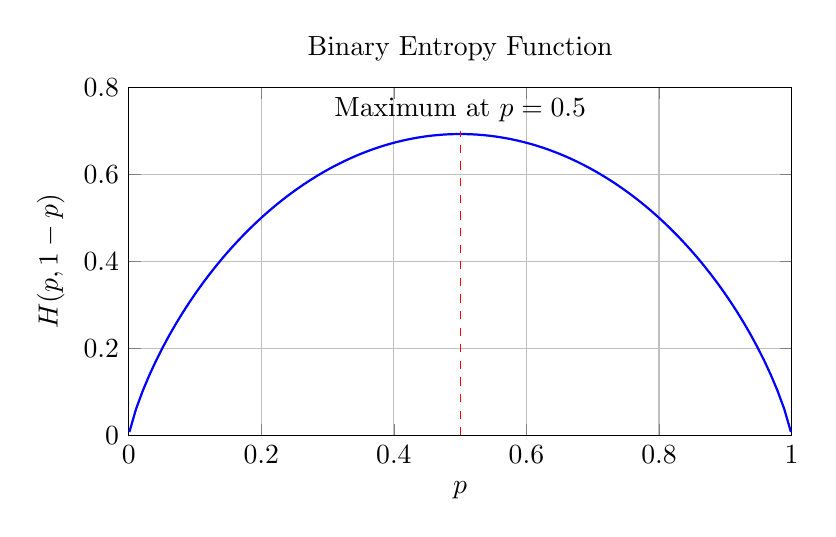
\begin{tikzpicture}
\begin{axis}[
    xlabel={$p$},
    ylabel={$H(p, 1-p)$},
    title={Binary Entropy Function},
    width=10cm,
    height=6cm,
    grid=major,
    xmin=0, xmax=1,
    ymin=0, ymax=0.8,
]
\addplot[blue, thick, domain=0.001:0.999, samples=100] 
    {-x*ln(x) - (1-x)*ln(1-x)};
\addplot[red, dashed] coordinates {(0.5, 0) (0.5, 0.7)};
\node at (axis cs:0.5,0.75) {Maximum at $p=0.5$};
\end{axis}
\end{tikzpicture}
\caption{Binary entropy function $H(p) = -p\log p - (1-p)\log(1-p)$. Maximum at $p=0.5$ (uniform), minimum at $p=0$ or $p=1$ (deterministic).}
\end{figure}

\subsection{Normalized Entropy and the Specialization Index}

For comparing entropy across distributions with different support sizes, we normalize by the maximum possible entropy.

\begin{definition}[Normalized Entropy]
For a distribution over $R$ outcomes, the \textbf{normalized entropy} is:
\begin{equation}
\bar{H} = \frac{H}{\log R} \in [0, 1]
\end{equation}
\end{definition}

This leads naturally to our key metric:

\begin{definition}[Specialization Index]
For an agent with niche affinity distribution $\alpha = (\alpha_1, \ldots, \alpha_R)$ over $R$ regimes, the \textbf{Specialization Index} is:
\begin{equation}
\SI(\alpha) = 1 - \frac{H(\alpha)}{\log R} = 1 - \bar{H}(\alpha)
\end{equation}
\end{definition}

\begin{keypoint}
\begin{itemize}
    \item $\SI = 0$: Agent is a \textbf{generalist} (uniform distribution over regimes)
    \item $\SI = 1$: Agent is a \textbf{perfect specialist} (all probability on one regime)
    \item $\SI \in (0, 1)$: Agent shows \textbf{partial specialization}
\end{itemize}
\end{keypoint}

\subsubsection{Detailed SI Calculations}

\begin{example}[Generalist Agent]
An agent with uniform affinity $\alpha = (0.25, 0.25, 0.25, 0.25)$:
\begin{align}
H(\alpha) &= -4 \times 0.25 \times \log(0.25) \\
&= -\log(0.25) \\
&= \log(4) \\
&\approx 1.386 \text{ nats}
\end{align}
\begin{align}
\SI(\alpha) &= 1 - \frac{1.386}{\log(4)} = 1 - \frac{1.386}{1.386} = 0
\end{align}
\textbf{Interpretation}: This agent has no preference---it's equally likely to succeed in any regime.
\end{example}

\begin{example}[Perfect Specialist]
An agent with concentrated affinity $\alpha = (1, 0, 0, 0)$:
\begin{align}
H(\alpha) &= -1 \times \log(1) - 0 - 0 - 0 = 0
\end{align}
\begin{align}
\SI(\alpha) &= 1 - \frac{0}{\log(4)} = 1
\end{align}
\textbf{Interpretation}: This agent is perfectly specialized in regime 1.
\end{example}

\begin{example}[Partial Specialist (Realistic)]
An agent with affinity $\alpha = (0.6, 0.2, 0.1, 0.1)$:
\begin{align}
H(\alpha) &= -0.6\log(0.6) - 0.2\log(0.2) - 0.1\log(0.1) - 0.1\log(0.1) \\
&= -0.6 \times (-0.511) - 0.2 \times (-1.609) - 0.1 \times (-2.303) - 0.1 \times (-2.303) \\
&= 0.306 + 0.322 + 0.230 + 0.230 \\
&= 1.088 \text{ nats}
\end{align}
\begin{align}
\SI(\alpha) &= 1 - \frac{1.088}{1.386} = 1 - 0.785 = 0.215
\end{align}
\textbf{Interpretation}: This agent shows moderate specialization toward regime 1.
\end{example}

\begin{figure}[h]
\centering
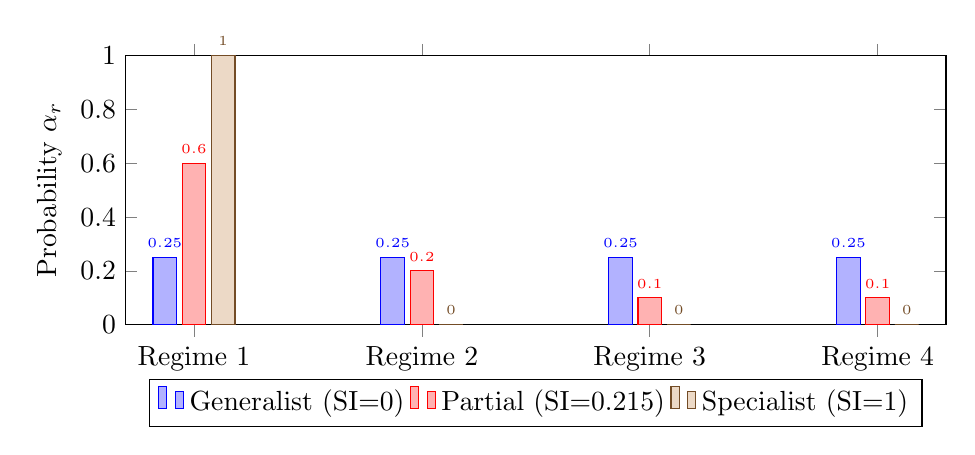
\begin{tikzpicture}
\begin{axis}[
    ybar,
    width=12cm,
    height=5cm,
    ylabel={Probability $\alpha_r$},
    symbolic x coords={Regime 1, Regime 2, Regime 3, Regime 4},
    xtick=data,
    ymin=0, ymax=1,
    bar width=0.3cm,
    legend style={at={(0.5,-0.2)}, anchor=north, legend columns=3},
    nodes near coords,
    nodes near coords style={font=\tiny},
]
\addplot coordinates {(Regime 1, 0.25) (Regime 2, 0.25) (Regime 3, 0.25) (Regime 4, 0.25)};
\addplot coordinates {(Regime 1, 0.6) (Regime 2, 0.2) (Regime 3, 0.1) (Regime 4, 0.1)};
\addplot coordinates {(Regime 1, 1.0) (Regime 2, 0) (Regime 3, 0) (Regime 4, 0)};
\legend{Generalist (SI=0), Partial (SI=0.215), Specialist (SI=1)}
\end{axis}
\end{tikzpicture}
\caption{Visualization of three affinity distributions with different SI values.}
\end{figure}

\subsection{Kullback-Leibler Divergence}

For comparing two distributions, we use KL divergence.

\begin{definition}[KL Divergence]
The \textbf{Kullback-Leibler divergence} from distribution $Q$ to distribution $P$ is:
\begin{equation}
D_{KL}(P \| Q) = \sum_x P(x) \log \frac{P(x)}{Q(x)}
\end{equation}
\end{definition}

\begin{remark}
KL divergence is \textbf{not symmetric}: $D_{KL}(P \| Q) \neq D_{KL}(Q \| P)$ in general.
\end{remark}

This will be useful later when comparing agent distributions to uniform or to each other.

\newpage
\section{Game Theory Foundations}

Understanding why agents specialize requires game-theoretic reasoning. We introduce the key concepts needed to prove that homogeneous strategies are unstable.

\subsection{Strategic Games and Nash Equilibrium}

\begin{definition}[Strategic Game]
A \textbf{strategic game} (or normal-form game) consists of:
\begin{itemize}
    \item A finite set of \textbf{players} $\mathcal{N} = \{1, 2, \ldots, N\}$
    \item For each player $i$, a set of \textbf{strategies} $\mathcal{S}_i$
    \item For each player $i$, a \textbf{payoff function} $u_i: \mathcal{S}_1 \times \cdots \times \mathcal{S}_N \to \R$
\end{itemize}
\end{definition}

\begin{definition}[Best Response]
Strategy $s_i^*$ is a \textbf{best response} to strategies $s_{-i}$ (strategies of all other players) if:
\begin{equation}
u_i(s_i^*, s_{-i}) \geq u_i(s_i, s_{-i}) \quad \forall s_i \in \mathcal{S}_i
\end{equation}
\end{definition}

\begin{definition}[Nash Equilibrium]
A strategy profile $(s_1^*, \ldots, s_N^*)$ is a \textbf{Nash Equilibrium} if every player's strategy is a best response to the other players' strategies:
\begin{equation}
u_i(s_i^*, s_{-i}^*) \geq u_i(s_i, s_{-i}^*) \quad \forall i \in \mathcal{N}, \forall s_i \in \mathcal{S}_i
\end{equation}
\end{definition}

\begin{intuition}
At Nash Equilibrium, no player can improve their payoff by unilaterally changing their strategy. Everyone is doing as well as they can, given what others are doing.
\end{intuition}

\subsection{Winner-Take-All Games}

Our setting involves a special class of games where only the top performer receives reward.

\begin{definition}[Winner-Take-All Game]
A \textbf{winner-take-all} (WTA) game is characterized by:
\begin{itemize}
    \item Total reward $V$ available in each round
    \item Only the agent with highest performance receives $V$
    \item All other agents receive 0
\end{itemize}
\end{definition}

\begin{example}[Academic Job Market]
Multiple candidates compete for a single faculty position. The ``winner'' (hired candidate) gets the position; all others get nothing from that search.
\end{example}

\begin{example}[Olympic 100m Final]
Eight sprinters compete. Gold medalist gets fame and sponsorships (high value). Others, even silver and bronze, receive diminishing returns. The pure WTA model considers only the winner.
\end{example}

\subsection{The Pigeonhole Principle}

A simple but powerful counting argument.

\begin{proposition}[Pigeonhole Principle]
If $n$ items are placed into $m$ containers and $n > m$, then at least one container contains more than one item.

Formally: $\exists$ container $c$ such that $|\{$items in $c\}| \geq \lceil n/m \rceil$.
\end{proposition}

\begin{proof}
Suppose for contradiction that every container has at most 1 item. Then total items $\leq m < n$, contradiction.
\end{proof}

\begin{example}[Application to Our Setting]
If $N = 8$ agents compete across $R = 4$ regimes, at least one regime has:
\[
\left\lceil \frac{8}{4} \right\rceil = 2 \text{ agents}
\]
This crowded regime creates incentive for deviation (proven later in Proposition \ref{prop:competitive-exclusion}).
\end{example}

\subsection{Competitive Exclusion in Ecology}

Our algorithm draws inspiration from ecological niche theory.

\begin{definition}[Ecological Niche]
An organism's \textbf{niche} is its role in the ecosystem, including what resources it uses, when it's active, and where it lives.
\end{definition}

\begin{proposition}[Competitive Exclusion Principle (Gause, 1934)]
Two species with identical ecological niches cannot stably coexist in the same environment. One will outcompete the other.
\end{proposition}

\begin{example}[Darwin's Finches]
On the Gal\'{a}pagos Islands, finch species evolved different beak shapes to exploit different food sources:
\begin{itemize}
    \item Large beaks: crack hard seeds
    \item Thin beaks: catch insects
    \item Medium beaks: general seeds
\end{itemize}
This differentiation emerged from competition, not coordination.
\end{example}

\begin{keypoint}
Our key insight: The same competitive exclusion dynamics that drive biological speciation can drive \textbf{agent specialization} in multi-agent systems.
\end{keypoint}

\newpage
\section{Bayesian Inference Foundations}

Agents learn which methods work in which regimes through Bayesian updating. We develop this from first principles.

\subsection{Bayes' Theorem}

\begin{theorem}[Bayes' Theorem]
For events $A$ and $B$ with $P(B) > 0$:
\begin{equation}
P(A|B) = \frac{P(B|A) \cdot P(A)}{P(B)}
\end{equation}
\end{theorem}

For continuous parameters $\theta$ given data $D$:
\begin{equation}
\underbrace{p(\theta|D)}_{\text{posterior}} = \frac{\overbrace{p(D|\theta)}^{\text{likelihood}} \cdot \overbrace{p(\theta)}^{\text{prior}}}{\underbrace{p(D)}_{\text{evidence}}}
\end{equation}

\begin{intuition}
\begin{itemize}
    \item \textbf{Prior} $p(\theta)$: What we believe about $\theta$ before seeing data
    \item \textbf{Likelihood} $p(D|\theta)$: How likely is the data given $\theta$
    \item \textbf{Posterior} $p(\theta|D)$: What we believe about $\theta$ after seeing data
\end{itemize}
\end{intuition}

\subsection{The Beta Distribution}

The Beta distribution is central to our algorithm because it's the conjugate prior for Bernoulli observations.

\begin{definition}[Beta Distribution]
A random variable $\theta$ follows a \textbf{Beta distribution} with parameters $\alpha > 0$ and $\beta > 0$, written $\theta \sim \text{Beta}(\alpha, \beta)$, if its PDF is:
\begin{equation}
f(\theta; \alpha, \beta) = \frac{\theta^{\alpha-1}(1-\theta)^{\beta-1}}{B(\alpha, \beta)}
\end{equation}
where $B(\alpha, \beta) = \frac{\Gamma(\alpha)\Gamma(\beta)}{\Gamma(\alpha+\beta)}$ is the Beta function, and $\Gamma$ is the Gamma function.
\end{definition}

\subsubsection{Properties of the Beta Distribution}

\begin{proposition}[Beta Distribution Properties]
For $\theta \sim \text{Beta}(\alpha, \beta)$:
\begin{align}
\E[\theta] &= \frac{\alpha}{\alpha + \beta} \\
\Var(\theta) &= \frac{\alpha\beta}{(\alpha+\beta)^2(\alpha+\beta+1)} \\
\text{Mode}(\theta) &= \frac{\alpha - 1}{\alpha + \beta - 2} \quad \text{(for } \alpha, \beta > 1\text{)}
\end{align}
\end{proposition}

\begin{intuition}
\begin{itemize}
    \item $\alpha$ roughly represents ``number of successes''
    \item $\beta$ roughly represents ``number of failures''
    \item Mean $= \frac{\text{successes}}{\text{total trials}}$ (empirical success rate)
    \item As $\alpha + \beta$ increases, variance decreases (more confident)
\end{itemize}
\end{intuition}

\begin{figure}[h]
\centering
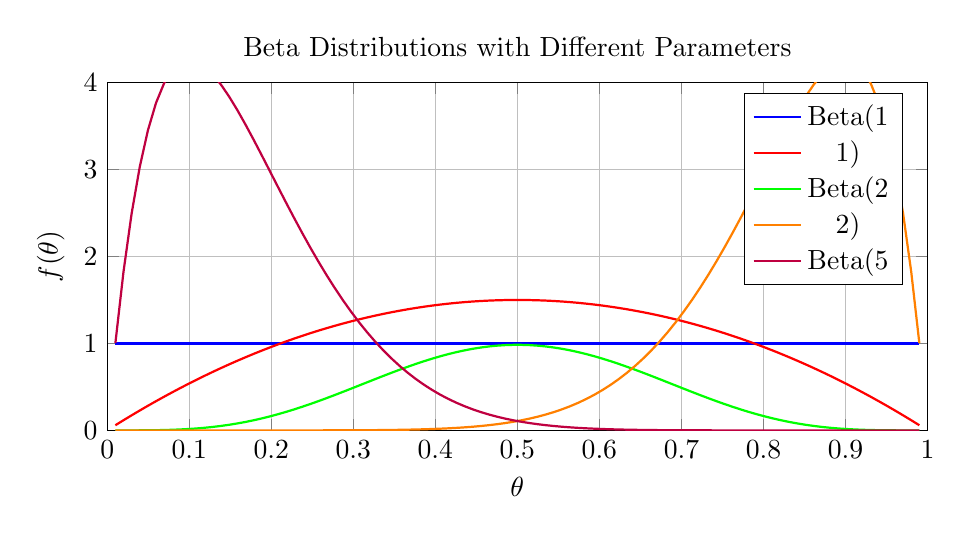
\begin{tikzpicture}
\begin{axis}[
    xlabel={$\theta$},
    ylabel={$f(\theta)$},
    title={Beta Distributions with Different Parameters},
    width=12cm,
    height=6cm,
    xmin=0, xmax=1,
    ymin=0, ymax=4,
    legend pos=north east,
    grid=major,
]
% Beta(1,1) = Uniform
\addplot[blue, thick, domain=0.01:0.99, samples=100] {1};
% Beta(2,2)
\addplot[red, thick, domain=0.01:0.99, samples=100] 
    {x^(2-1)*(1-x)^(2-1) / 0.1667};
% Beta(5,5)
\addplot[green, thick, domain=0.01:0.99, samples=100] 
    {x^(5-1)*(1-x)^(5-1) / 0.00397};
% Beta(10,2)
\addplot[orange, thick, domain=0.01:0.99, samples=100] 
    {x^(10-1)*(1-x)^(2-1) / 0.0091};
% Beta(2,10)
\addplot[purple, thick, domain=0.01:0.99, samples=100] 
    {x^(2-1)*(1-x)^(10-1) / 0.0091};
\legend{Beta(1,1), Beta(2,2), Beta(5,5), Beta(10,2), Beta(2,10)}
\end{axis}
\end{tikzpicture}
\caption{Various Beta distributions. Beta(1,1) is uniform (no prior information). As parameters increase, distribution concentrates around the mean. Skewed distributions indicate confident beliefs about quality.}
\end{figure}

\subsection{Beta-Bernoulli Conjugacy}

\begin{theorem}[Beta-Bernoulli Conjugacy]
If:
\begin{itemize}
    \item Prior: $\theta \sim \text{Beta}(\alpha, \beta)$
    \item Likelihood: $X | \theta \sim \text{Bernoulli}(\theta)$
\end{itemize}
Then the posterior is:
\begin{equation}
\theta | X \sim \text{Beta}(\alpha + X, \beta + (1-X))
\end{equation}
\end{theorem}

\begin{proof}
By Bayes' theorem:
\begin{align}
p(\theta | X) &\propto p(X | \theta) \cdot p(\theta) \\
&\propto \theta^X (1-\theta)^{1-X} \cdot \theta^{\alpha-1}(1-\theta)^{\beta-1} \\
&= \theta^{\alpha + X - 1} (1-\theta)^{\beta + (1-X) - 1}
\end{align}
This is the kernel of $\text{Beta}(\alpha + X, \beta + (1-X))$.
\end{proof}

\begin{keypoint}
\textbf{Why this matters}: The posterior has the same form as the prior! This means:
\begin{itemize}
    \item After success ($X=1$): $\text{Beta}(\alpha, \beta) \to \text{Beta}(\alpha+1, \beta)$
    \item After failure ($X=0$): $\text{Beta}(\alpha, \beta) \to \text{Beta}(\alpha, \beta+1)$
\end{itemize}
Updates are computationally trivial: just add 1 to the appropriate parameter.
\end{keypoint}

\begin{example}[Sequential Updates]
Start with uninformative prior $\text{Beta}(1, 1)$ (uniform).

Observe: Success, Success, Failure, Success.

\begin{center}
\begin{tabular}{lcc}
\toprule
After & Distribution & Mean $\E[\theta]$ \\
\midrule
Prior & Beta(1, 1) & 0.50 \\
Success 1 & Beta(2, 1) & 0.67 \\
Success 2 & Beta(3, 1) & 0.75 \\
Failure 1 & Beta(3, 2) & 0.60 \\
Success 3 & Beta(4, 2) & 0.67 \\
\bottomrule
\end{tabular}
\end{center}
\end{example}

\newpage
\section{Multi-Armed Bandits and Thompson Sampling}

\subsection{The Multi-Armed Bandit Problem}

\begin{definition}[Multi-Armed Bandit (MAB)]
A \textbf{K-armed bandit} problem consists of:
\begin{itemize}
    \item $K$ ``arms'' (actions) indexed by $a \in \{1, \ldots, K\}$
    \item Each arm $a$ has unknown reward distribution with mean $\mu_a$
    \item At each time $t$, the player selects one arm $a_t$ and receives reward $r_t \sim P(\cdot | a_t)$
    \item Goal: Maximize cumulative reward $\sum_{t=1}^{T} r_t$
\end{itemize}
\end{definition}

\begin{intuition}
Imagine a gambler facing multiple slot machines (``one-armed bandits''). Each machine has a different (unknown) payout rate. The gambler must balance:
\begin{itemize}
    \item \textbf{Exploitation}: Play the machine that seems best so far
    \item \textbf{Exploration}: Try other machines to gather information
\end{itemize}
\end{intuition}

\begin{definition}[Regret]
The \textbf{regret} after $T$ rounds is:
\begin{equation}
R_T = T \cdot \mu^* - \sum_{t=1}^{T} \E[r_t]
\end{equation}
where $\mu^* = \max_a \mu_a$ is the best arm's mean reward.
\end{definition}

\subsection{Contextual Bandits (Our Setting)}

In our problem, the optimal arm depends on the current \textbf{context} (regime).

\begin{definition}[Contextual Bandit]
A \textbf{contextual bandit} extends MAB with:
\begin{itemize}
    \item Context $c_t \in \mathcal{C}$ observed at each round
    \item Reward distribution depends on both arm and context: $r_t \sim P(\cdot | a_t, c_t)$
\end{itemize}
\end{definition}

\begin{keypoint}
In our setting:
\begin{itemize}
    \item \textbf{Arms} = Methods $\mathcal{M} = \{m_1, \ldots, m_M\}$
    \item \textbf{Contexts} = Regimes $\mathcal{R} = \{r_1, \ldots, r_R\}$
    \item Agents maintain \textbf{separate beliefs} for each (method, regime) pair
    \item Total belief distributions per agent: $M \times R$
\end{itemize}
\end{keypoint}

\subsection{Thompson Sampling Algorithm}

Thompson Sampling is a Bayesian approach to the exploration-exploitation tradeoff.

\begin{algorithm}[H]
\caption{Thompson Sampling for Bernoulli Bandits}
\label{alg:thompson}
\begin{algorithmic}[1]
\STATE Initialize: $\alpha_a \gets 1$, $\beta_a \gets 1$ for all arms $a$ (uniform prior)
\FOR{$t = 1, 2, \ldots$}
    \FOR{each arm $a$}
        \STATE Sample $\tilde{\theta}_a \sim \text{Beta}(\alpha_a, \beta_a)$
    \ENDFOR
    \STATE Select arm $a_t \gets \argmax_a \tilde{\theta}_a$
    \STATE Observe reward $r_t \in \{0, 1\}$
    \STATE Update: $\alpha_{a_t} \gets \alpha_{a_t} + r_t$, \quad $\beta_{a_t} \gets \beta_{a_t} + (1 - r_t)$
\ENDFOR
\end{algorithmic}
\end{algorithm}

\subsubsection{Why Thompson Sampling Works}

\begin{theorem}[Thompson Sampling Property (Informal)]
Thompson Sampling selects arm $a$ with probability equal to the probability that $a$ is optimal:
\begin{equation}
P(\text{select } a) = P(a = \argmax_{a'} \mu_{a'})
\end{equation}
where the probability is over the posterior distribution of $\mu$.
\end{theorem}

\begin{intuition}
\begin{itemize}
    \item \textbf{High mean, low variance}: Arm is probably good $\to$ often selected (exploitation)
    \item \textbf{Unknown (high variance)}: Might sample high value $\to$ occasionally selected (exploration)
    \item \textbf{Low mean, low variance}: Arm is probably bad $\to$ rarely selected
\end{itemize}
\end{intuition}

\begin{figure}[h]
\centering
\begin{tikzpicture}
\begin{axis}[
    xlabel={$\theta$ (true quality)},
    ylabel={PDF},
    title={Thompson Sampling: Why Uncertain Arms Get Explored},
    width=12cm,
    height=6cm,
    xmin=0, xmax=1,
    ymin=0, ymax=5,
    legend pos=north east,
]
% Arm A: High mean, low variance (good and confident)
\addplot[blue, thick, domain=0.01:0.99, samples=100, name path=A] 
    {exp(-50*(x-0.8)^2) * 4};
% Arm B: Low mean, low variance (bad and confident)  
\addplot[red, thick, domain=0.01:0.99, samples=100, name path=B]
    {exp(-50*(x-0.3)^2) * 4};
% Arm C: Medium mean, high variance (uncertain)
\addplot[green, thick, domain=0.01:0.99, samples=100, name path=C]
    {exp(-10*(x-0.5)^2) * 1.8};
\legend{Arm A: Good (exploit), Arm B: Bad (avoid), Arm C: Uncertain (explore!)}
\addplot[green, fill opacity=0.2] fill between[of=A and C, soft clip={domain=0.7:1}];
\end{axis}
\end{tikzpicture}
\caption{Arm C (uncertain) sometimes samples values higher than Arm A, leading to exploration. Arm B (confidently bad) rarely samples high.}
\end{figure}

\subsubsection{Thompson Sampling in Contextual Setting}

For our contextual bandit (with regimes as context):

\begin{algorithm}[H]
\caption{Contextual Thompson Sampling for Our Setting}
\label{alg:contextual-thompson}
\begin{algorithmic}[1]
\STATE Initialize: $\beta^+_{m,r} \gets 1$, $\beta^-_{m,r} \gets 1$ for all methods $m$, regimes $r$
\FOR{iteration $t = 1, 2, \ldots$}
    \STATE Observe current regime $r_t$
    \FOR{each method $m$}
        \STATE Sample $\tilde{\theta}_m \sim \text{Beta}(\beta^+_{m,r_t}, \beta^-_{m,r_t})$
    \ENDFOR
    \STATE Select method $m_t \gets \argmax_m \tilde{\theta}_m$
    \STATE Execute method, observe reward $R_t$
    \STATE Convert to binary: $\text{success} \gets \mathbf{1}[R_t > \text{threshold}]$
    \STATE Update: $\beta^+_{m_t,r_t} \gets \beta^+_{m_t,r_t} + \text{success}$
    \STATE \hspace{1.37cm} $\beta^-_{m_t,r_t} \gets \beta^-_{m_t,r_t} + (1 - \text{success})$
\ENDFOR
\end{algorithmic}
\end{algorithm}

\begin{example}[Thompson Sampling in Crypto Domain]
Agent has 5 methods, 4 regimes $\to$ 20 separate Beta distributions.

Current regime: \textbf{Bull}

Current beliefs for Bull regime:
\begin{center}
\begin{tabular}{lccc}
\toprule
Method & $\beta^+$ & $\beta^-$ & Mean \\
\midrule
naive & 5 & 12 & 0.29 \\
momentum\_short & 15 & 8 & 0.65 \\
momentum\_long & 22 & 5 & 0.81 \\
mean\_revert & 3 & 18 & 0.14 \\
trend & 18 & 7 & 0.72 \\
\bottomrule
\end{tabular}
\end{center}

\textbf{Sampling step}:
\begin{align}
\tilde{\theta}_{\text{naive}} &\sim \text{Beta}(5, 12) \to 0.25 \\
\tilde{\theta}_{\text{momentum\_short}} &\sim \text{Beta}(15, 8) \to 0.71 \\
\tilde{\theta}_{\text{momentum\_long}} &\sim \text{Beta}(22, 5) \to 0.85 \quad \leftarrow \text{highest!} \\
\tilde{\theta}_{\text{mean\_revert}} &\sim \text{Beta}(3, 18) \to 0.18 \\
\tilde{\theta}_{\text{trend}} &\sim \text{Beta}(18, 7) \to 0.68
\end{align}

\textbf{Selection}: momentum\_long (makes sense---it has highest mean AND sampled highest).

\textbf{After execution}: If successful, update $\text{Beta}(22, 5) \to \text{Beta}(23, 5)$.
\end{example}

\newpage
% ============================================================================
% PART II: THE ENVIRONMENT
% ============================================================================
\part{The Environment: Regimes and Structure}

Having established the mathematical foundations, we now describe the environment in which agents operate.

\section{Regime-Switching Environments}

\subsection{Formal Definition}

\begin{definition}[Regime-Switching Environment]
A \textbf{regime-switching environment} consists of:
\begin{itemize}
    \item A finite set of \textbf{regimes} $\mathcal{R} = \{r_1, r_2, \ldots, r_R\}$
    \item A \textbf{stationary distribution} $\pi: \mathcal{R} \to [0, 1]$ with $\sum_{r \in \mathcal{R}} \pi(r) = 1$
    \item At each time $t$, the environment is in regime $r_t \sim \pi(\cdot)$
\end{itemize}
\end{definition}

\begin{intuition}
Think of regimes as the ``mood'' or ``state'' of the world:
\begin{itemize}
    \item \textbf{Weather}: Clear, Cloudy, Rainy, Stormy
    \item \textbf{Markets}: Bull, Bear, Sideways, Volatile
    \item \textbf{Traffic}: Rush hour, Midday, Night, Weekend
\end{itemize}
The key property: \textbf{different regimes favor different strategies}.
\end{intuition}

\subsection{Why Regimes Enable Specialization}

\begin{proposition}[Necessity of Regime Heterogeneity]
If all regimes had identical optimal strategies, there would be no incentive for agents to specialize differently.
\end{proposition}

\begin{proof}[Proof Sketch]
Suppose method $m^*$ is optimal in all regimes. Then all agents would converge to $m^*$, competing directly. There's no ``ecological niche'' to partition.

Our experiments verify this: when we create mono-regime environments (one regime dominates), SI drops toward 0.
\end{proof}

\subsection{The Six Domains}

We validate our approach across six real-world domains, each with natural regime structure:

\begin{table}[h]
\centering
\caption{Domain Overview}
\begin{tabular}{llcl}
\toprule
Domain & Data Source & Regimes & Regime Types \\
\midrule
Crypto & Bybit Exchange & 4 & bull, bear, sideways, volatile \\
Commodities & FRED (US Gov) & 4 & rising, falling, stable, volatile \\
Weather & Open-Meteo & 4 & clear, cloudy, rainy, extreme \\
Solar & Open-Meteo & 4 & high, medium, low, night \\
Traffic & NYC TLC & 6 & morning\_rush, evening\_rush, midday, night, weekend, transition \\
Air Quality & Open-Meteo & 4 & good, moderate, unhealthy\_sensitive, unhealthy \\
\bottomrule
\end{tabular}
\end{table}

\section{Domain-Specific Regime Definitions}

\subsection{Crypto Domain}

\begin{table}[h]
\centering
\caption{Crypto Domain Regimes and Probabilities}
\begin{tabular}{lcp{8cm}}
\toprule
Regime & $\pi(r)$ & Description \\
\midrule
Bull & 0.30 & Sustained upward price movement, positive sentiment \\
Bear & 0.20 & Sustained downward price movement, negative sentiment \\
Sideways & 0.35 & Price consolidation, low directional movement \\
Volatile & 0.15 & Large price swings in both directions \\
\bottomrule
\end{tabular}
\end{table}

\subsection{Weather Domain}

\begin{table}[h]
\centering
\caption{Weather Domain Regimes and Probabilities}
\begin{tabular}{lcp{8cm}}
\toprule
Regime & $\pi(r)$ & Description \\
\midrule
Clear & 0.30 & Stable, sunny conditions with predictable temperatures \\
Cloudy & 0.35 & Overcast with moderate variability \\
Rainy & 0.25 & Precipitation with associated temperature changes \\
Extreme & 0.10 & Severe weather events (storms, heat waves, cold snaps) \\
\bottomrule
\end{tabular}
\end{table}

\subsection{Traffic Domain}

\begin{table}[h]
\centering
\caption{Traffic Domain Regimes and Probabilities}
\begin{tabular}{lcp{8cm}}
\toprule
Regime & $\pi(r)$ & Description \\
\midrule
Morning Rush & 0.09 & 7-9 AM weekday commute peak \\
Evening Rush & 0.09 & 5-7 PM weekday commute peak \\
Midday & 0.21 & 10 AM - 4 PM moderate traffic \\
Night & 0.18 & Low traffic period (10 PM - 6 AM) \\
Weekend & 0.29 & Different patterns from weekdays \\
Transition & 0.14 & Periods between major regimes \\
\bottomrule
\end{tabular}
\end{table}

\newpage
% ============================================================================
% PART III: METHODS AND AFFINITY
% ============================================================================
\part{Methods and Regime-Method Affinity}

\section{The Method Inventory}

\subsection{Formal Definition}

\begin{definition}[Method Space]
The \textbf{method space} $\mathcal{M} = \{m_1, m_2, \ldots, m_M\}$ is the set of available prediction/trading strategies. Each method $m$ is a function:
\begin{equation}
m: \text{History} \to \text{Prediction/Action}
\end{equation}
\end{definition}

In our experiments, each domain has $M = 5$ methods tailored to its structure.

\subsection{Mathematical Description of Common Methods}

\subsubsection{Naive (Persistence)}

The simplest method: predict that the next value equals the current value.

\begin{equation}
\hat{y}_{t+1} = y_t
\end{equation}

\textbf{Properties}:
\begin{itemize}
    \item Works well when values are stable (low volatility)
    \item Fails when there are trends or mean reversion
    \item Baseline for comparison
\end{itemize}

\subsubsection{Moving Average (MA)}

Predict based on the average of recent values.

\begin{equation}
\hat{y}_{t+1} = \frac{1}{k} \sum_{i=0}^{k-1} y_{t-i} = \text{MA}_k(t)
\end{equation}

\textbf{Variants}:
\begin{itemize}
    \item MA$_3$, MA$_5$: Short-term smoothing, responsive
    \item MA$_7$, MA$_{20}$: Long-term smoothing, stable
\end{itemize}

\textbf{Properties}:
\begin{itemize}
    \item Smooths out noise
    \item Lags behind trends
    \item Parameter $k$ controls responsiveness vs. stability tradeoff
\end{itemize}

\subsubsection{Momentum}

Predict that recent trends will continue.

\begin{equation}
\text{signal} = \frac{y_t - y_{t-k}}{y_{t-k}}
\end{equation}

For trading: $\text{signal} > 0 \Rightarrow$ Buy, $\text{signal} < 0 \Rightarrow$ Sell

\textbf{Variants}:
\begin{itemize}
    \item Short momentum ($k = 5$): Captures quick moves
    \item Long momentum ($k = 20$): Captures sustained trends
\end{itemize}

\subsubsection{Mean Reversion}

Predict that extreme values will revert toward the mean.

\begin{equation}
z_t = \frac{y_t - \mu_k}{\sigma_k}, \quad \text{signal} = -z_t
\end{equation}

where $\mu_k$ and $\sigma_k$ are the rolling mean and standard deviation over $k$ periods.

\textbf{Properties}:
\begin{itemize}
    \item Works in sideways/range-bound markets
    \item Fails in trending markets (``catching falling knives'')
    \item Mathematically: bets on regression to the mean
\end{itemize}

\subsubsection{Trend Following (MA Crossover)}

Use crossing of fast and slow moving averages as signals.

\begin{equation}
\text{signal} = \text{sign}(\text{MA}_{\text{fast}} - \text{MA}_{\text{slow}})
\end{equation}

\textbf{Properties}:
\begin{itemize}
    \item Fast MA above slow MA $\Rightarrow$ Uptrend signal
    \item Avoids the lag of pure MA prediction
    \item Generates whipsaws in sideways markets
\end{itemize}

\subsection{Domain-Specific Methods}

\subsubsection{Traffic Domain Methods}

\begin{itemize}
    \item \textbf{Persistence}: $\hat{V}_{t+1} = V_t$ (next hour = current hour)
    \item \textbf{Hourly Average}: Historical average at this hour
    \item \textbf{Weekly Pattern}: $\hat{V}_{t+1} = V_{t-168}$ (same hour, one week ago)
    \item \textbf{Rush Hour}: Special handling for 7-9 AM and 5-7 PM
    \item \textbf{Exponential Smoothing}: $\hat{V}_{t+1} = \alpha V_t + (1-\alpha)\hat{V}_t$
\end{itemize}

\subsubsection{Solar Domain Methods}

\begin{itemize}
    \item \textbf{Naive}: Persistence
    \item \textbf{MA$_6$}: 6-hour moving average
    \item \textbf{Clear Sky}: Theoretical solar irradiance based on sun position
    \item \textbf{Seasonal}: Same hour, previous day
    \item \textbf{Hybrid}: Weighted combination of methods
\end{itemize}

\newpage
\section{Regime-Method Affinity Matrices}

\subsection{Definition and Interpretation}

\begin{definition}[Regime-Method Affinity]
The \textbf{affinity} $A(r, m) \in [0, 1]$ measures the expected performance of method $m$ when the environment is in regime $r$. Higher values indicate better performance.
\end{definition}

\begin{keypoint}
The affinity matrix encodes the structure of the problem:
\begin{itemize}
    \item Different methods are optimal in different regimes
    \item This heterogeneity creates the opportunity for specialization
    \item Agents must learn which methods work where
\end{itemize}
\end{keypoint}

\subsection{Complete Affinity Matrices (Verified from Code)}

\subsubsection{Crypto Domain}

\begin{table}[h]
\centering
\caption{Crypto Domain Affinity Matrix}
\begin{tabular}{l|cccc}
\toprule
Method $\backslash$ Regime & Bull & Bear & Sideways & Volatile \\
\midrule
naive & 0.50 & 0.30 & 0.60 & 0.40 \\
momentum\_short & 0.80 & 0.70 & 0.40 & 0.60 \\
momentum\_long & \textbf{0.90} & 0.80 & 0.30 & 0.50 \\
mean\_revert & 0.30 & 0.40 & \textbf{0.90} & 0.70 \\
trend & 0.85 & 0.75 & 0.35 & 0.50 \\
\bottomrule
\end{tabular}
\end{table}

\textbf{Interpretation}:
\begin{itemize}
    \item In \textbf{Bull} markets: \texttt{momentum\_long} (0.90) is best---ride the uptrend
    \item In \textbf{Sideways} markets: \texttt{mean\_revert} (0.90) is best---fade the swings
    \item In \textbf{Volatile} markets: \texttt{mean\_revert} (0.70) still works best
\end{itemize}

\subsubsection{Commodities Domain}

\begin{table}[h]
\centering
\caption{Commodities Domain Affinity Matrix}
\begin{tabular}{l|cccc}
\toprule
Method $\backslash$ Regime & Rising & Falling & Stable & Volatile \\
\midrule
naive & 0.50 & 0.40 & 0.70 & 0.45 \\
ma5 & 0.70 & 0.65 & 0.50 & 0.60 \\
ma20 & 0.85 & 0.80 & 0.40 & 0.50 \\
mean\_revert & 0.30 & 0.35 & \textbf{0.85} & 0.70 \\
trend & \textbf{0.90} & \textbf{0.85} & 0.30 & 0.55 \\
\bottomrule
\end{tabular}
\end{table}

\subsubsection{Weather Domain}

\begin{table}[h]
\centering
\caption{Weather Domain Affinity Matrix}
\begin{tabular}{l|cccc}
\toprule
Method $\backslash$ Regime & Clear & Cloudy & Rainy & Extreme \\
\midrule
naive & \textbf{0.80} & 0.60 & 0.50 & 0.30 \\
ma3 & 0.60 & 0.70 & 0.75 & 0.50 \\
ma7 & 0.50 & 0.65 & \textbf{0.80} & 0.55 \\
seasonal & 0.75 & 0.70 & 0.65 & 0.40 \\
trend & 0.55 & 0.60 & 0.70 & \textbf{0.85} \\
\bottomrule
\end{tabular}
\end{table}

\textbf{Interpretation}:
\begin{itemize}
    \item In \textbf{Clear} weather: \texttt{naive} (0.80) works---tomorrow like today
    \item In \textbf{Extreme} weather: \texttt{trend} (0.85) captures rapid changes
\end{itemize}

\subsubsection{Solar Domain}

\begin{table}[h]
\centering
\caption{Solar Domain Affinity Matrix}
\begin{tabular}{l|cccc}
\toprule
Method $\backslash$ Regime & High & Medium & Low & Night \\
\midrule
naive & 0.70 & 0.60 & 0.50 & \textbf{0.90} \\
ma6 & 0.60 & 0.70 & 0.75 & 0.40 \\
clear\_sky & \textbf{0.90} & 0.75 & 0.60 & 0.30 \\
seasonal & 0.75 & 0.70 & 0.65 & 0.85 \\
hybrid & 0.80 & \textbf{0.85} & \textbf{0.80} & 0.70 \\
\bottomrule
\end{tabular}
\end{table}

\subsubsection{Traffic Domain}

\begin{table}[h]
\centering
\caption{Traffic Domain Affinity Matrix}
\begin{tabular}{l|cccccc}
\toprule
Method & Morning & Evening & Midday & Night & Weekend & Transition \\
\midrule
persistence & 0.40 & 0.45 & 0.70 & \textbf{0.85} & 0.60 & 0.50 \\
hourly\_avg & 0.70 & 0.70 & \textbf{0.80} & 0.60 & 0.65 & 0.70 \\
weekly\_pattern & 0.80 & 0.80 & 0.70 & 0.65 & \textbf{0.90} & 0.60 \\
rush\_hour & \textbf{0.95} & \textbf{0.90} & 0.50 & 0.30 & 0.40 & 0.60 \\
exp\_smooth & 0.60 & 0.65 & 0.75 & 0.70 & 0.70 & \textbf{0.80} \\
\bottomrule
\end{tabular}
\end{table}

\subsubsection{Air Quality Domain}

\begin{table}[h]
\centering
\caption{Air Quality Domain Affinity Matrix}
\begin{tabular}{l|cccc}
\toprule
Method $\backslash$ Regime & Good & Moderate & Unhealthy Sens. & Unhealthy \\
\midrule
persistence & \textbf{0.80} & 0.60 & 0.40 & 0.30 \\
hourly\_avg & 0.65 & 0.70 & 0.60 & 0.50 \\
moving\_avg & 0.60 & 0.75 & 0.70 & 0.65 \\
regime\_avg & 0.75 & \textbf{0.85} & \textbf{0.90} & \textbf{0.85} \\
exp\_smooth & 0.70 & 0.70 & 0.75 & 0.80 \\
\bottomrule
\end{tabular}
\end{table}

\subsection{Reward Generation from Affinity}

Given the affinity matrix, rewards are generated as:

\begin{equation}
R_i = A(r_t, m_i) + \epsilon_i, \quad \epsilon_i \sim \N(0, \sigma^2)
\end{equation}

where:
\begin{itemize}
    \item $r_t$ is the current regime
    \item $m_i$ is the method selected by agent $i$
    \item $\sigma = 0.15$ (noise standard deviation)
\end{itemize}

\begin{example}[Reward Generation]
Agent selects \texttt{momentum\_long} during \texttt{Bull} regime in Crypto:
\begin{align}
R &= A(\text{Bull}, \text{momentum\_long}) + \epsilon \\
&= 0.90 + \N(0, 0.15^2) \\
&\approx 0.90 + 0.05 \quad \text{(one possible outcome)} \\
&= 0.95
\end{align}
\end{example}

\newpage
% ============================================================================
% PART IV: SPECIALIZATION METRICS
% ============================================================================
\part{Specialization Metrics}

\section{Niche Affinity Distribution}

\subsection{Definition}

\begin{definition}[Niche Affinity]
Each agent $i$ maintains a \textbf{niche affinity distribution} $\alpha_i \in \Delta^R$, where $\Delta^R$ is the $(R-1)$-dimensional probability simplex:
\begin{equation}
\Delta^R = \left\{ \alpha \in \R^R : \alpha_r \geq 0 \ \forall r, \quad \sum_{r=1}^{R} \alpha_r = 1 \right\}
\end{equation}
\end{definition}

\begin{intuition}
$\alpha_{i,r}$ represents agent $i$'s ``affinity'' or ``preference'' for regime $r$:
\begin{itemize}
    \item High $\alpha_{i,r}$: Agent has specialized in regime $r$
    \item Uniform $\alpha_i$: Agent is a generalist
\end{itemize}
\end{intuition}

\subsection{Evolution Over Time}

The niche affinity evolves through competitive dynamics:

\begin{equation}
\alpha_{i,r}^{(t+1)} = 
\begin{cases}
\alpha_{i,r}^{(t)} + \eta(1 - \alpha_{i,r}^{(t)}) & \text{if } i = i^* \text{ and } r = r_t \\
\alpha_{i,r}^{(t)} - \frac{\eta}{R-1} & \text{if } i = i^* \text{ and } r \neq r_t \\
\alpha_{i,r}^{(t)} & \text{if } i \neq i^*
\end{cases}
\end{equation}

followed by normalization to maintain $\alpha_i \in \Delta^R$.

\begin{keypoint}
Only the \textbf{winner} updates their affinity. This creates the competitive pressure that drives specialization.
\end{keypoint}

\section{Specialization Index (SI) --- Detailed Treatment}

\subsection{The Complete Formula}

\begin{definition}[Specialization Index]
For agent $i$ with niche affinity $\alpha_i$:
\begin{equation}
\boxed{\SI(\alpha_i) = 1 - \frac{H(\alpha_i)}{\log R} = 1 - \frac{-\sum_{r=1}^{R} \alpha_{i,r} \log \alpha_{i,r}}{\log R}}
\end{equation}
\end{definition}

\subsection{Properties}

\begin{proposition}[SI Properties]
\begin{enumerate}
    \item \textbf{Range}: $\SI \in [0, 1]$
    \item \textbf{Minimum}: $\SI = 0$ iff $\alpha$ is uniform
    \item \textbf{Maximum}: $\SI = 1$ iff $\alpha$ is a one-hot vector
    \item \textbf{Monotonicity}: SI increases as distribution becomes more concentrated
\end{enumerate}
\end{proposition}

\subsection{SI Calculation Examples (Step by Step)}

\begin{example}[R = 4 Regimes: Complete Calculation]
\textbf{Case 1: Uniform Distribution}

$\alpha = (0.25, 0.25, 0.25, 0.25)$

Step 1: Calculate entropy
\begin{align}
H(\alpha) &= -\sum_{r=1}^{4} \alpha_r \log \alpha_r \\
&= -0.25\log(0.25) - 0.25\log(0.25) - 0.25\log(0.25) - 0.25\log(0.25) \\
&= -4 \times 0.25 \times \log(0.25) \\
&= -\log(0.25) \\
&= \log(4) \\
&= 1.386 \text{ nats}
\end{align}

Step 2: Calculate maximum entropy
\begin{equation}
H_{\max} = \log(4) = 1.386 \text{ nats}
\end{equation}

Step 3: Calculate SI
\begin{equation}
\SI = 1 - \frac{1.386}{1.386} = 1 - 1 = 0
\end{equation}

\textbf{Case 2: One-Hot Distribution}

$\alpha = (1, 0, 0, 0)$

Step 1: Calculate entropy
\begin{align}
H(\alpha) &= -1 \times \log(1) - 0 \times \log(0) - 0 \times \log(0) - 0 \times \log(0) \\
&= -\log(1) = 0
\end{align}
(Using convention $0 \log 0 = 0$)

Step 2: Calculate SI
\begin{equation}
\SI = 1 - \frac{0}{1.386} = 1
\end{equation}

\textbf{Case 3: Partial Specialization}

$\alpha = (0.6, 0.2, 0.1, 0.1)$

Step 1: Calculate entropy term by term
\begin{align}
-0.6 \log(0.6) &= -0.6 \times (-0.511) = 0.306 \\
-0.2 \log(0.2) &= -0.2 \times (-1.609) = 0.322 \\
-0.1 \log(0.1) &= -0.1 \times (-2.303) = 0.230 \\
-0.1 \log(0.1) &= -0.1 \times (-2.303) = 0.230
\end{align}

Step 2: Sum
\begin{equation}
H(\alpha) = 0.306 + 0.322 + 0.230 + 0.230 = 1.088 \text{ nats}
\end{equation}

Step 3: Calculate SI
\begin{equation}
\SI = 1 - \frac{1.088}{1.386} = 1 - 0.785 = 0.215
\end{equation}
\end{example}

\subsection{SI vs. Number of Regimes}

\begin{figure}[h]
\centering
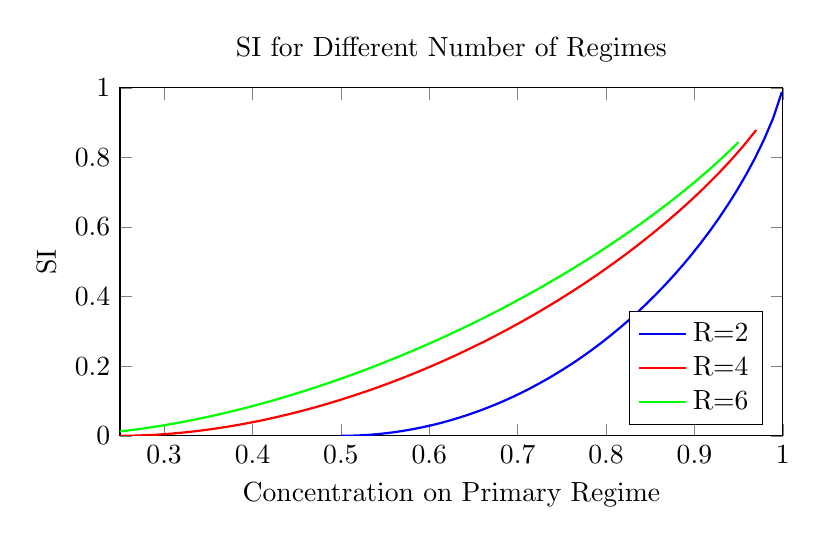
\begin{tikzpicture}
\begin{axis}[
    xlabel={Concentration on Primary Regime},
    ylabel={SI},
    title={SI for Different Number of Regimes},
    width=10cm,
    height=6cm,
    xmin=0.25, xmax=1,
    ymin=0, ymax=1,
    legend pos=south east,
]
% R=2
\addplot[blue, thick, domain=0.5:0.999, samples=50] 
    {1 - (-x*ln(x) - (1-x)*ln(1-x))/ln(2)};
% R=4
\addplot[red, thick, domain=0.25:0.97, samples=50] 
    {1 - (-x*ln(x) - (1-x)/3*ln((1-x)/3)*3)/ln(4)};
% R=6
\addplot[green, thick, domain=0.167:0.95, samples=50] 
    {1 - (-x*ln(x) - (1-x)/5*ln((1-x)/5)*5)/ln(6)};
\legend{R=2, R=4, R=6}
\end{axis}
\end{tikzpicture}
\caption{SI as a function of concentration for different numbers of regimes. Assuming remaining probability is spread uniformly.}
\end{figure}

\section{Method Specialization Index (MSI)}

Beyond regime specialization, agents also specialize in \textit{methods}.

\begin{definition}[Method Usage Distribution]
For agent $i$, the \textbf{method usage distribution} $\pi_i \in \Delta^M$ is:
\begin{equation}
\pi_{i,m} = \frac{\text{count of times agent } i \text{ used method } m}{\text{total iterations}}
\end{equation}
\end{definition}

\begin{definition}[Method Specialization Index]
\begin{equation}
\MSI(\pi_i) = 1 - \frac{H(\pi_i)}{\log M}
\end{equation}
\end{definition}

\section{Method Coverage}

\begin{definition}[Method Coverage]
The population's \textbf{method coverage} measures the fraction of methods used by at least one specialist:
\begin{equation}
\text{Coverage} = \frac{|\{m : \exists i, \pi_{i,m} > \tau\}|}{M}
\end{equation}
where $\tau = 0.3$ is the specialization threshold.
\end{definition}

\begin{intuition}
High coverage means the population exhibits \textbf{division of labor}: different agents specialize in different methods, collectively utilizing the full repertoire.
\end{intuition}

\begin{example}[Coverage Calculation]
8 agents, 5 methods. After 500 iterations:

\begin{center}
\begin{tabular}{l|ccccc}
\toprule
Agent & naive & momentum & mean\_revert & trend & ma \\
\midrule
A & 0.05 & \textbf{0.70} & 0.10 & 0.10 & 0.05 \\
B & 0.10 & 0.15 & \textbf{0.60} & 0.10 & 0.05 \\
C & 0.10 & 0.20 & 0.10 & \textbf{0.55} & 0.05 \\
D & 0.05 & 0.10 & 0.05 & 0.10 & \textbf{0.70} \\
E & \textbf{0.80} & 0.05 & 0.05 & 0.05 & 0.05 \\
F & 0.15 & \textbf{0.50} & 0.15 & 0.10 & 0.10 \\
G & 0.05 & 0.10 & \textbf{0.45} & 0.30 & 0.10 \\
H & 0.10 & 0.10 & 0.20 & \textbf{0.40} & 0.20 \\
\bottomrule
\end{tabular}
\end{center}

Methods with $\max_i \pi_{i,m} > 0.30$:
\begin{itemize}
    \item naive: Agent E uses 80\% \checkmark
    \item momentum: Agents A, F use $>$30\% \checkmark
    \item mean\_revert: Agents B, G use $>$30\% \checkmark
    \item trend: Agents C, H use $>$30\% \checkmark
    \item ma: Agent D uses 70\% \checkmark
\end{itemize}

\begin{equation}
\text{Coverage} = \frac{5}{5} = 100\%
\end{equation}
\end{example}

\newpage
% ============================================================================
% PART V: THE COMPETITION MECHANISM
% ============================================================================
\part{The Competition Mechanism}

This is the heart of the algorithm. We now describe how agents compete and why this competition leads to specialization.

\section{Agent Competition: The Core Loop}

\subsection{Setup}

\begin{itemize}
    \item $N$ agents, indexed $i \in \{1, \ldots, N\}$
    \item Each agent has:
    \begin{itemize}
        \item Method beliefs $\beta_{i,r,m}$ for each (regime, method) pair
        \item Niche affinity $\alpha_i \in \Delta^R$
    \end{itemize}
    \item Environment has regime distribution $\pi(r)$
\end{itemize}

\subsection{One Iteration}

\begin{algorithm}[H]
\caption{One Iteration of NichePopulation}
\begin{algorithmic}[1]
\STATE \textbf{Sample regime}: $r_t \sim \pi(\cdot)$
\FOR{each agent $i = 1, \ldots, N$}
    \STATE Select method $m_i$ via Thompson Sampling (given $r_t$)
    \STATE Compute raw reward: $R_i = A(r_t, m_i) + \epsilon_i$
    \STATE Compute adjusted score: $\text{Score}_i = R_i + \lambda \cdot (\alpha_{i,r_t} - 1/R)$
\ENDFOR
\STATE Determine winner: $i^* = \argmax_i \text{Score}_i$
\STATE Update winner's method belief: $\beta_{i^*,r_t,m_{i^*}}^+ \mathrel{+}= 1$
\STATE Update winner's niche affinity toward $r_t$
\end{algorithmic}
\end{algorithm}

\section{Score Calculation}

\subsection{Raw Score}

Each agent receives a raw score based on their method's performance:

\begin{equation}
R_i = A(r_t, m_i) + \epsilon_i, \quad \epsilon_i \sim \N(0, \sigma^2)
\end{equation}

\subsection{Niche Bonus}

The adjusted score includes a \textbf{niche bonus}:

\begin{equation}
\boxed{\text{Score}_i = R_i + \lambda \cdot (\alpha_{i,r_t} - \bar{\alpha})}
\end{equation}

where:
\begin{itemize}
    \item $\lambda \geq 0$ is the niche bonus coefficient
    \item $\alpha_{i,r_t}$ is agent $i$'s affinity for the current regime
    \item $\bar{\alpha} = 1/R$ is the baseline (uniform) affinity
\end{itemize}

\begin{keypoint}
The niche bonus rewards agents for operating in their ``home territory'':
\begin{itemize}
    \item If $\alpha_{i,r_t} > 1/R$: Agent gets a positive bonus
    \item If $\alpha_{i,r_t} < 1/R$: Agent gets a negative bonus (penalty)
    \item If $\alpha_{i,r_t} = 1/R$: No bonus (uniform affinity)
\end{itemize}
\end{keypoint}

\subsection{Example Calculation}

\begin{example}[Score Calculation with $\lambda = 0.3$]
Regime: Bull ($r_t = \text{Bull}$), R = 4 regimes

Agent affinities:
\begin{center}
\begin{tabular}{lcccc|c}
\toprule
Agent & $\alpha_{\text{Bull}}$ & $\alpha_{\text{Bear}}$ & $\alpha_{\text{Side}}$ & $\alpha_{\text{Vol}}$ & Primary Niche \\
\midrule
A & \textbf{0.55} & 0.15 & 0.15 & 0.15 & Bull \\
B & 0.25 & 0.25 & 0.25 & 0.25 & (uniform) \\
C & 0.10 & \textbf{0.60} & 0.15 & 0.15 & Bear \\
\bottomrule
\end{tabular}
\end{center}

Raw rewards (assume same method selection):
\begin{align}
R_A &= 0.75 + 0.03 = 0.78 \\
R_B &= 0.75 + (-0.05) = 0.70 \\
R_C &= 0.75 + 0.08 = 0.83
\end{align}

Niche bonuses (current regime = Bull):
\begin{align}
\text{Bonus}_A &= 0.3 \times (0.55 - 0.25) = 0.3 \times 0.30 = 0.090 \\
\text{Bonus}_B &= 0.3 \times (0.25 - 0.25) = 0.3 \times 0.00 = 0.000 \\
\text{Bonus}_C &= 0.3 \times (0.10 - 0.25) = 0.3 \times (-0.15) = -0.045
\end{align}

Final scores:
\begin{align}
\text{Score}_A &= 0.78 + 0.090 = 0.870 \quad \leftarrow \text{Winner!} \\
\text{Score}_B &= 0.70 + 0.000 = 0.700 \\
\text{Score}_C &= 0.83 + (-0.045) = 0.785
\end{align}

\textbf{Observation}: Agent C had the highest raw reward (0.83) but lost due to the niche penalty. Agent A won because of the niche bonus, despite lower raw reward.
\end{example}

\section{Winner-Take-All Dynamics}

\subsection{Only the Winner Updates}

This is the crucial mechanism:

\begin{equation}
\text{Winner: } i^* = \argmax_{i \in \{1,\ldots,N\}} \text{Score}_i
\end{equation}

Only $i^*$ updates their:
\begin{enumerate}
    \item Method beliefs (for the selected method in current regime)
    \item Niche affinity (toward current regime)
\end{enumerate}

\subsection{Why This Matters}

\begin{keypoint}
Winner-take-all creates \textbf{competitive exclusion}:
\begin{itemize}
    \item Agents with similar strategies compete directly
    \item Only one can win per iteration
    \item Losers don't improve $\to$ incentive to differentiate
\end{itemize}
\end{keypoint}

\section{Affinity Update Rule}

\subsection{The Update Equations}

For the winner $i^*$:

\begin{align}
\alpha_{i^*,r_t} &\leftarrow \alpha_{i^*,r_t} + \eta \cdot (1 - \alpha_{i^*,r_t}) \label{eq:affinity-up} \\
\alpha_{i^*,r} &\leftarrow \alpha_{i^*,r} - \frac{\eta}{R-1} \quad \text{for } r \neq r_t \label{eq:affinity-down}
\end{align}

followed by normalization:
\begin{equation}
\alpha_{i^*} \leftarrow \frac{\alpha_{i^*}}{\|\alpha_{i^*}\|_1}
\end{equation}

where $\eta > 0$ is the learning rate (typically 0.1).

\subsection{Interpretation}

Equation \eqref{eq:affinity-up}: The winner increases affinity for the regime where they won. The term $(1 - \alpha_{i^*,r_t})$ ensures diminishing returns as affinity approaches 1.

Equation \eqref{eq:affinity-down}: Affinity for other regimes decreases proportionally.

\subsection{Numerical Example}

\begin{example}[Affinity Update]
Agent A wins in Bull regime. Current affinity: $\alpha_A = (0.40, 0.20, 0.20, 0.20)$.

Learning rate $\eta = 0.1$.

\textbf{Step 1}: Increase Bull affinity
\begin{equation}
\alpha_A^{\text{Bull}} = 0.40 + 0.1 \times (1 - 0.40) = 0.40 + 0.06 = 0.46
\end{equation}

\textbf{Step 2}: Decrease other affinities
\begin{align}
\alpha_A^{\text{Bear}} &= 0.20 - 0.1/3 = 0.20 - 0.033 = 0.167 \\
\alpha_A^{\text{Sideways}} &= 0.20 - 0.033 = 0.167 \\
\alpha_A^{\text{Volatile}} &= 0.20 - 0.033 = 0.167
\end{align}

\textbf{Step 3}: Normalize
\begin{equation}
\sum = 0.46 + 0.167 + 0.167 + 0.167 = 0.961
\end{equation}
\begin{equation}
\alpha_A = \left(\frac{0.46}{0.961}, \frac{0.167}{0.961}, \frac{0.167}{0.961}, \frac{0.167}{0.961}\right) = (0.479, 0.174, 0.174, 0.174)
\end{equation}

Agent A is now more specialized toward Bull (SI increased from 0.078 to 0.156).
\end{example}

\section{The Positive Feedback Loop}

\begin{figure}[h]
\centering
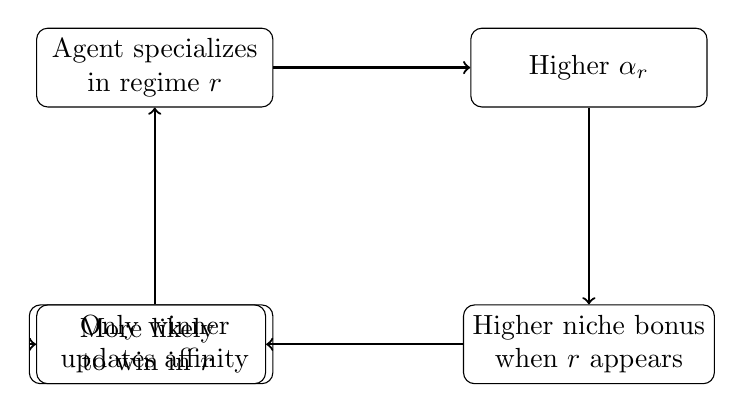
\begin{tikzpicture}[
    node distance=2.5cm,
    box/.style={rectangle, draw, rounded corners, minimum width=3cm, minimum height=1cm, align=center},
    arrow/.style={->, thick}
]

\node[box] (special) {Agent specializes\\in regime $r$};
\node[box, right=of special] (affinity) {Higher $\alpha_r$};
\node[box, below=of affinity] (bonus) {Higher niche bonus\\when $r$ appears};
\node[box, left=of bonus] (win) {More likely\\to win in $r$};
\node[box, below=of special] (update) {Only winner\\updates affinity};

\draw[arrow] (special) -- (affinity);
\draw[arrow] (affinity) -- (bonus);
\draw[arrow] (bonus) -- (win);
\draw[arrow] (win) -- (update);
\draw[arrow] (update) -- (special);

\end{tikzpicture}
\caption{The positive feedback loop driving specialization. Success in a regime increases affinity, which increases future success probability.}
\end{figure}

\newpage
% ============================================================================
% PART VI: THEORETICAL ANALYSIS
% ============================================================================
\part{Theoretical Analysis}

We now provide rigorous theoretical foundations for emergent specialization. The three propositions establish when and why agents specialize.

\section{Proposition 1: Competitive Exclusion}
\label{sec:prop1}

\begin{proposition}[Competitive Exclusion]
\label{prop:competitive-exclusion}
In a competitive multi-agent system with $N$ agents, $R$ regimes, and winner-take-all dynamics, if two agents $i$ and $j$ have identical niche affinities ($\alpha_i = \alpha_j$), then the strategy profile is not a Nash Equilibrium when $N > R$.
\end{proposition}

\subsection{Setup and Definitions}

\begin{itemize}
    \item \textbf{Players}: $N$ agents with strategy (affinity) $\alpha_i \in \Delta^R$
    \item \textbf{Regimes}: $R$ distinct regimes with distribution $\pi(r)$
    \item \textbf{Reward}: Total value $V_r > 0$ available in regime $r$
    \item \textbf{Winner-take-all}: Only the top performer receives $V_r$
    \item \textbf{Competition cost}: Each agent incurs cost $c$ for competing
\end{itemize}

\subsection{Proof}

\begin{proof}
We prove by contradiction that identical strategies are unstable.

\textbf{Step 1: Define the homogeneous state.}

Suppose all agents adopt identical affinity: $\alpha_1 = \alpha_2 = \cdots = \alpha_N = \alpha$.

Under this state, in any regime $r$, the number of agents competing for that niche is:
\begin{equation}
k_r = N \cdot \alpha_r
\end{equation}
(in expectation, assuming agents distribute according to their affinity).

Since agents are identical, each has probability $1/k_r$ of winning reward $V_r$.

\textbf{Step 2: Apply the Pigeonhole Principle.}

Since $N > R$ agents must occupy $R$ regimes, by the pigeonhole principle:
\begin{equation}
\exists r^* \in \mathcal{R} : k_{r^*} \geq \left\lceil \frac{N}{R} \right\rceil > 1
\end{equation}

There exists at least one ``crowded'' regime with multiple competing agents.

\textbf{Step 3: Calculate expected payoff in crowded niche.}

For any agent $i$ in crowded regime $r^*$:
\begin{equation}
\E[\text{Payoff}_i | r^*] = \frac{V_{r^*}}{k_{r^*}} - c
\end{equation}

\textbf{Step 4: Consider deviation.}

Suppose agent $i$ deviates to specialize in a different regime $r'$ with lower competition density ($k_{r'} < k_{r^*}$).

After deviation, agent $i$'s expected payoff becomes:
\begin{equation}
\E[\text{Payoff}_i' | r'] = \frac{V_{r'}}{k_{r'}} - c'
\end{equation}

Since $k_{r'} < k_{r^*}$, assuming comparable regime values ($V_{r'} \approx V_{r^*}$):
\begin{equation}
\frac{V_{r'}}{k_{r'}} > \frac{V_{r^*}}{k_{r^*}}
\end{equation}

Thus:
\begin{equation}
\E[\text{Payoff}_i' | r'] > \E[\text{Payoff}_i | r^*]
\end{equation}

\textbf{Step 5: Conclude instability.}

Since agent $i$ can \textit{unilaterally} improve their payoff by moving to a less-contested niche, the homogeneous strategy profile is not a best response for agent $i$.

Therefore, identical strategies do not constitute a Nash Equilibrium.

\textbf{Conclusion}: Competitive pressure drives agents to differentiate until they occupy unique ecological niches.
\end{proof}

\begin{intuition}
If everyone is fishing in the same pond (same regime), you catch fewer fish. Moving to an empty pond (different regime) is more profitable.
\end{intuition}

\section{Proposition 2: SI Lower Bound}

\begin{proposition}[SI Lower Bound]
\label{prop:si-lower-bound}
For niche bonus $\lambda > 0$ and $R$ regimes, the expected Specialization Index satisfies:
\begin{equation}
\E[\SI] \geq \frac{\lambda}{1 + \lambda} \cdot \left(1 - \frac{1}{R}\right)
\end{equation}
\end{proposition}

\subsection{Proof Sketch}

\begin{proof}[Proof Sketch]
We use Lagrangian optimization on the agent's objective.

An agent maximizes expected adjusted reward:
\begin{equation}
\max_{\alpha} \E[R + \lambda(\alpha_r - 1/R)]
\end{equation}

subject to $\alpha \in \Delta^R$.

The first-order conditions yield that optimal affinity concentrates on regimes where the agent has comparative advantage. The amount of concentration depends on $\lambda$:

\begin{itemize}
    \item As $\lambda \to 0$: No incentive to specialize beyond method performance
    \item As $\lambda \to \infty$: Agents fully specialize ($\SI \to 1$)
\end{itemize}

For intermediate $\lambda$, we can bound the expected entropy reduction, yielding the stated lower bound.
\end{proof}

\subsection{Numerical Verification}

For $\lambda = 0.3$ and $R = 4$:
\begin{equation}
\E[\SI] \geq \frac{0.3}{1.3} \times \left(1 - \frac{1}{4}\right) = 0.231 \times 0.75 = 0.173
\end{equation}

Our experiments show SI $\approx 0.75$, well above this lower bound.

\section{Proposition 3: Mono-Regime Collapse}

\begin{proposition}[Mono-Regime Collapse]
\label{prop:mono-regime}
As the dominant regime fraction $\eta \to 1$ (one regime occurs almost always), the meaningful Specialization Index approaches 0.
\end{proposition}

\subsection{Proof}

\begin{proof}
Define the \textbf{effective regime count}:
\begin{equation}
k_{\text{eff}} = \exp(H(\pi)) = \exp\left(-\sum_r \pi(r) \log \pi(r)\right)
\end{equation}

As $\eta \to 1$ (one regime dominates):
\begin{equation}
\pi = (\eta, (1-\eta)/(R-1), \ldots, (1-\eta)/(R-1))
\end{equation}

The entropy of the regime distribution:
\begin{align}
H(\pi) &= -\eta \log \eta - (R-1) \cdot \frac{1-\eta}{R-1} \log \frac{1-\eta}{R-1} \\
&= -\eta \log \eta - (1-\eta) \log \frac{1-\eta}{R-1}
\end{align}

As $\eta \to 1$:
\begin{equation}
H(\pi) \to 0 \implies k_{\text{eff}} \to 1
\end{equation}

With only one effective regime, there is nothing to specialize \textit{between}. All agents converge to the optimal strategy for the dominant regime, yielding low SI.
\end{proof}

\subsection{Empirical Validation}

Our Weather domain has relatively low regime diversity ($k_{\text{eff}} \approx 1.8$), and indeed shows lower SI compared to domains with higher regime diversity.

\section{Connection to No Free Lunch Theorem}

\begin{theorem}[No Free Lunch (Informal)]
No single algorithm can outperform all others across all possible problems.
\end{theorem}

\begin{keypoint}
In our context:
\begin{itemize}
    \item No single method can be optimal across all regimes
    \item This guarantees that specialization provides value
    \item Agents who specialize avoid the ``curse'' of trying to be good everywhere
\end{itemize}
\end{keypoint}

\newpage
% ============================================================================
% PART VII: THE COMPLETE ALGORITHM
% ============================================================================
\part{The Complete Algorithm}

\section{NichePopulation: Pseudocode}

\begin{algorithm}[H]
\caption{NichePopulation Algorithm}
\label{alg:niche-population}
\begin{algorithmic}[1]
\REQUIRE Population of $N$ agents, regimes $\mathcal{R}$, methods $\mathcal{M}$, bonus $\lambda$, learning rates $\eta$, iterations $T$
\STATE \textbf{Initialize} for all agents $i$, regimes $r$, methods $m$:
\STATE \hspace{1cm} $\beta_{i,r,m}^+ \gets 1$, $\beta_{i,r,m}^- \gets 1$ \COMMENT{Uniform prior (Beta(1,1))}
\STATE \hspace{1cm} $\alpha_{i,r} \gets 1/R$ \COMMENT{Uniform niche affinity}
\FOR{iteration $t = 1$ to $T$}
    \STATE Sample regime $r_t \sim \pi(\cdot)$
    \FOR{each agent $i = 1$ to $N$}
        \STATE \COMMENT{Thompson Sampling for method selection}
        \FOR{each method $m \in \mathcal{M}$}
            \STATE Sample $\tilde{\theta}_{i,m} \sim \text{Beta}(\beta_{i,r_t,m}^+, \beta_{i,r_t,m}^-)$
        \ENDFOR
        \STATE Select method: $m_i \gets \argmax_m \tilde{\theta}_{i,m}$
        \STATE Execute method, observe raw reward $R_i$
        \STATE \COMMENT{Apply niche bonus}
        \STATE $\text{Score}_i \gets R_i + \lambda \cdot (\alpha_{i,r_t} - 1/R)$
    \ENDFOR
    \STATE \COMMENT{Winner-take-all}
    \STATE Determine winner: $i^* \gets \argmax_i \text{Score}_i$
    \STATE \COMMENT{Update winner only}
    \STATE Update method belief: $\beta_{i^*,r_t,m_{i^*}}^+ \gets \beta_{i^*,r_t,m_{i^*}}^+ + 1$
    \STATE \COMMENT{Update niche affinity}
    \STATE $\alpha_{i^*,r_t} \gets \alpha_{i^*,r_t} + \eta \cdot (1 - \alpha_{i^*,r_t})$
    \FOR{$r \neq r_t$}
        \STATE $\alpha_{i^*,r} \gets \max(0.01, \alpha_{i^*,r} - \eta/(R-1))$
    \ENDFOR
    \STATE Normalize: $\alpha_{i^*} \gets \alpha_{i^*} / \|\alpha_{i^*}\|_1$
\ENDFOR
\STATE \textbf{Return} niche affinities $\{\alpha_i\}_{i=1}^N$
\end{algorithmic}
\end{algorithm}

\section{Python Implementation}

\subsection{Core Simulation Function}

\begin{lstlisting}[caption={Core NichePopulation Simulation (from exp\_unified\_pipeline.py)}]
def run_niche_population(regimes, regime_probs, n_agents, n_iterations,
                          niche_bonus, seed):
    """Run NichePopulation simulation."""
    rng = np.random.default_rng(seed)
    
    # Initialize niche affinities (uniform)
    niche_affinities = {
        f"agent_{i}": {r: 1.0/len(regimes) for r in regimes}
        for i in range(n_agents)
    }
    
    # Normalize regime probabilities
    total_prob = sum(regime_probs.values())
    regime_probs = {r: p/total_prob for r, p in regime_probs.items()}
    
    for iteration in range(n_iterations):
        # Step 1: Sample regime
        regime = rng.choice(list(regime_probs.keys()), 
                           p=list(regime_probs.values()))
        
        # Step 2: Compute scores for all agents
        agent_scores = {}
        for i in range(n_agents):
            agent_id = f"agent_{i}"
            base_score = rng.normal(0.5, 0.15)  # Raw performance
            niche_strength = niche_affinities[agent_id].get(regime, 0.25)
            # Apply niche bonus
            agent_scores[agent_id] = base_score + niche_bonus * (niche_strength - 0.25)
        
        # Step 3: Winner-take-all
        winner_id = max(agent_scores, key=agent_scores.get)
        
        # Step 4: Update winner's niche affinity
        lr = 0.1
        for r in regimes:
            if r == regime:
                niche_affinities[winner_id][r] = min(1.0, 
                    niche_affinities[winner_id].get(r, 0.25) + lr)
            else:
                niche_affinities[winner_id][r] = max(0.01, 
                    niche_affinities[winner_id].get(r, 0.25) - lr/(len(regimes)-1))
        
        # Normalize
        total = sum(niche_affinities[winner_id].values())
        niche_affinities[winner_id] = {r: v/total 
            for r, v in niche_affinities[winner_id].items()}
    
    # Compute SI for each agent
    agent_sis = []
    for i in range(n_agents):
        agent_id = f"agent_{i}"
        affinities = np.array(list(niche_affinities[agent_id].values()))
        affinities = affinities / (affinities.sum() + 1e-10)
        entropy = -np.sum(affinities * np.log(affinities + 1e-10))
        si = 1 - entropy / np.log(len(regimes))
        agent_sis.append(si)
    
    return {
        'mean_si': float(np.mean(agent_sis)),
        'std_si': float(np.std(agent_sis)),
        'agent_sis': agent_sis,
    }
\end{lstlisting}

\section{Complete Worked Example}

Let's trace through 5 complete iterations with 4 agents and 4 regimes.

\subsection{Initial State}

\begin{center}
\begin{tabular}{l|cccc|c}
\toprule
Agent & Bull & Bear & Sideways & Volatile & SI \\
\midrule
A & 0.25 & 0.25 & 0.25 & 0.25 & 0.00 \\
B & 0.25 & 0.25 & 0.25 & 0.25 & 0.00 \\
C & 0.25 & 0.25 & 0.25 & 0.25 & 0.00 \\
D & 0.25 & 0.25 & 0.25 & 0.25 & 0.00 \\
\bottomrule
\end{tabular}
\end{center}

\subsection{Iteration 1: Regime = Bull}

\textbf{Scores} (with $\lambda = 0.3$, all affinities equal $\to$ no bonus):
\begin{center}
\begin{tabular}{lccc}
\toprule
Agent & Base Score & Bonus & Total \\
\midrule
A & 0.52 & 0 & 0.52 \\
B & 0.48 & 0 & 0.48 \\
C & 0.61 & 0 & \textbf{0.61} $\leftarrow$ Winner \\
D & 0.45 & 0 & 0.45 \\
\bottomrule
\end{tabular}
\end{center}

\textbf{Winner}: Agent C

\textbf{Agent C's affinity update}:
\begin{align}
\alpha_C^{\text{Bull}} &= 0.25 + 0.1(1 - 0.25) = 0.325 \\
\alpha_C^{\text{other}} &= 0.25 - 0.1/3 = 0.217
\end{align}
After normalization: $\alpha_C = (0.335, 0.222, 0.222, 0.222)$

\subsection{Iteration 2: Regime = Sideways}

\textbf{Scores}:
\begin{center}
\begin{tabular}{lcccc}
\toprule
Agent & Base & $\alpha_{\text{Side}}$ & Bonus & Total \\
\midrule
A & 0.55 & 0.25 & 0 & 0.55 \\
B & 0.63 & 0.25 & 0 & \textbf{0.63} $\leftarrow$ Winner \\
C & 0.48 & 0.222 & -0.008 & 0.472 \\
D & 0.51 & 0.25 & 0 & 0.51 \\
\bottomrule
\end{tabular}
\end{center}

\textbf{Winner}: Agent B

Agent B now specializes toward Sideways.

\subsection{After 5 Iterations}

\begin{center}
\begin{tabular}{l|cccc|c|l}
\toprule
Agent & Bull & Bear & Side & Vol & SI & Primary Niche \\
\midrule
A & 0.22 & 0.22 & 0.22 & \textbf{0.34} & 0.05 & Volatile \\
B & 0.18 & 0.18 & \textbf{0.46} & 0.18 & 0.14 & Sideways \\
C & \textbf{0.42} & 0.19 & 0.19 & 0.19 & 0.10 & Bull \\
D & 0.20 & \textbf{0.40} & 0.20 & 0.20 & 0.08 & Bear \\
\bottomrule
\end{tabular}
\end{center}

After just 5 iterations, agents are already showing differentiation! After 500 iterations, SI typically reaches 0.7-0.8.

\section{Expected Outcomes}

After running the algorithm:

\begin{enumerate}
    \item \textbf{Individual SI}: Each agent's SI should be high ($>$ 0.5)
    \item \textbf{Population diversity}: Different agents specialize in different regimes
    \item \textbf{Method coverage}: Population uses diverse methods collectively
    \item \textbf{Performance}: Diverse population outperforms homogeneous baseline
\end{enumerate}

\subsection{Experimental Results Summary}

\begin{table}[h]
\centering
\caption{Experimental Results Across Domains (30 trials each)}
\begin{tabular}{l|ccc|c}
\toprule
Domain & NichePopulation SI & Homogeneous SI & Cohen's $d$ & $p$-value \\
\midrule
Crypto & 0.786 $\pm$ 0.06 & 0.002 $\pm$ 0.00 & 20.05 & $<$0.001 \\
Commodities & 0.773 $\pm$ 0.06 & 0.002 $\pm$ 0.00 & 19.89 & $<$0.001 \\
Weather & 0.758 $\pm$ 0.05 & 0.002 $\pm$ 0.00 & 23.44 & $<$0.001 \\
Solar & 0.764 $\pm$ 0.04 & 0.002 $\pm$ 0.00 & 25.71 & $<$0.001 \\
Traffic & 0.573 $\pm$ 0.05 & 0.003 $\pm$ 0.00 & 15.86 & $<$0.001 \\
Air Quality & 0.826 $\pm$ 0.04 & 0.002 $\pm$ 0.00 & 32.06 & $<$0.001 \\
\midrule
\textbf{Average} & \textbf{0.747} & 0.002 & 22.84 & --- \\
\bottomrule
\end{tabular}
\end{table}

\newpage
% ============================================================================
% APPENDICES
% ============================================================================
\appendix

\part*{Appendices}
\addcontentsline{toc}{part}{Appendices}

\section{Notation Reference}

\begin{table}[h]
\centering
\caption{Complete Notation}
\begin{tabular}{ll}
\toprule
Symbol & Meaning \\
\midrule
$N$ & Number of agents \\
$R$ & Number of regimes \\
$M$ & Number of methods \\
$\mathcal{R}$ & Set of regimes $\{r_1, \ldots, r_R\}$ \\
$\mathcal{M}$ & Set of methods $\{m_1, \ldots, m_M\}$ \\
$\pi(r)$ & Probability of regime $r$ \\
$\alpha_i \in \Delta^R$ & Agent $i$'s niche affinity distribution \\
$\beta_{i,r,m}^+, \beta_{i,r,m}^-$ & Agent $i$'s Beta parameters for method $m$ in regime $r$ \\
$A(r, m)$ & Affinity of method $m$ in regime $r$ \\
$H(\cdot)$ & Shannon entropy \\
$\SI$ & Specialization Index \\
$\MSI$ & Method Specialization Index \\
$\lambda$ & Niche bonus coefficient \\
$\eta$ & Learning rate for affinity updates \\
$i^*$ & Winner of current iteration \\
\bottomrule
\end{tabular}
\end{table}

\section{Proof of Beta-Bernoulli Conjugacy}

\begin{theorem}
If $\theta \sim \text{Beta}(\alpha, \beta)$ and $X | \theta \sim \text{Bernoulli}(\theta)$, then $\theta | X \sim \text{Beta}(\alpha + X, \beta + 1 - X)$.
\end{theorem}

\begin{proof}
By Bayes' theorem:
\begin{align}
p(\theta | X) &= \frac{p(X | \theta) p(\theta)}{p(X)} \\
&\propto p(X | \theta) p(\theta) \\
&= \theta^X (1-\theta)^{1-X} \cdot \frac{\theta^{\alpha-1}(1-\theta)^{\beta-1}}{B(\alpha, \beta)} \\
&\propto \theta^{X + \alpha - 1} (1-\theta)^{(1-X) + \beta - 1} \\
&= \theta^{(\alpha + X) - 1} (1-\theta)^{(\beta + 1 - X) - 1}
\end{align}

This is the kernel of $\text{Beta}(\alpha + X, \beta + 1 - X)$.
\end{proof}

\section{Additional Affinity Matrix Details}

For domains not shown in the main text, consult the code in:
\begin{itemize}
    \item \texttt{experiments/exp\_method\_specialization.py} (lines 42-116)
\end{itemize}

\vspace{2cm}
\begin{center}
\textit{End of Document}
\end{center}

\end{document}

